\subsection{Design System Components}\label{sds_button}
An important part of the implementation of a design system are the components. As described in chapter \ref{sds-component}, the components are created using the Lit framework. To see a complete example of a component constructed with design tokens and documented with the storybook, the example of the button component of the \ac{SDS} is presented in this chapter. \\
The components use TypeScript to take advantage of custom decorators. The decorators provided by Lit further simplify the boilerplate code for creating a web component. \\
\lstinputlisting[linerange={1-4},firstnumber=1,caption={Initialization of \ac{SDS} button component},label=ButtonInit]{../Code/src/components/button.component.ts}
In listing \ref{ButtonInit}, the component is initialised with the \texttt{@customElement} decorator by passing the tag name as a string and appending it to an ES6 class. For it to work properly, the class must extend the LitElement class. When everything has been implemented as described, the web component is registered and can be used with the defined tag, in this case \texttt{<saas-button>}. \\
In order to see something when the web component just created is used, it must implement the render method. This method expects a \texttt{TemplateResult}. 
\lstinputlisting[linerange={19-26},firstnumber=19,caption={Rendering of \ac{SDS} button component},label=ButtonRender]{../Code/src/components/button.component.ts}
Lit element provides the import of a \texttt{html} string literal that can be used to construct the \texttt{TemplateResult} expected by the render function. With this functionality, Lit provides an efficient way to respond to variable changes and intelligently update the DOM. \\
Properties also make use of custom decorators and declare properties on web components by writing \texttt{@property} in front of a class attribute (line 19-20, Listing \ref{ButtonRender}). Thus, Lit Element implements change detection and adds automatic type conversion. For a detailed description of the capabilities of this decorator, see the documentation. Whenever the property value of the created button web component changes, the constructed template string reacts to these changes and updates the displayed template accordingly. \\
Last but not least, the web component must use the defined design tokens. Since these tokens are defined by \ac{CSS} variables, they can simply be consumed as follows: 
\lstinputlisting[linerange={5-20},firstnumber=5,caption={Styles of \ac{SDS} button component},label=ButtonStyles]{../Code/src/components/button.component.ts}
The Lit Element framework implements a static property of the \texttt{styles} to its classes. To make it work properly, a string literal \texttt{css} is used to convert a string into the required \texttt{CSSResult} type. In this way it would be possible to consume design tokens via input properties, but to simply manipulate design tokens in one place, the components of \ac{SDS} will use \ac{CSS} variables. In this way, it is possible to customise certain tokens throughout the design system by adapting these tokens. Each component in the \ac{SDS} will use the defined tokens. Line 7-9 in listing \ref{ButtonStyles} shows an example of the use of design tokens for the button component in the \ac{SDS}. \\
Finally, the button component is displayed in Storybook, the documentation tool for \ac{SDS}. Limited to the time frame of this elaboration, the documentation is kept short. Figure \ref{storybook_button} is an example of what the documentation of \ac{SDS} components may look like. A full version of documentation as in other mature design systems will have to be added in a subsequent development of \ac{SDS}. \\
\begin{figure}[htbp]
    \centerline{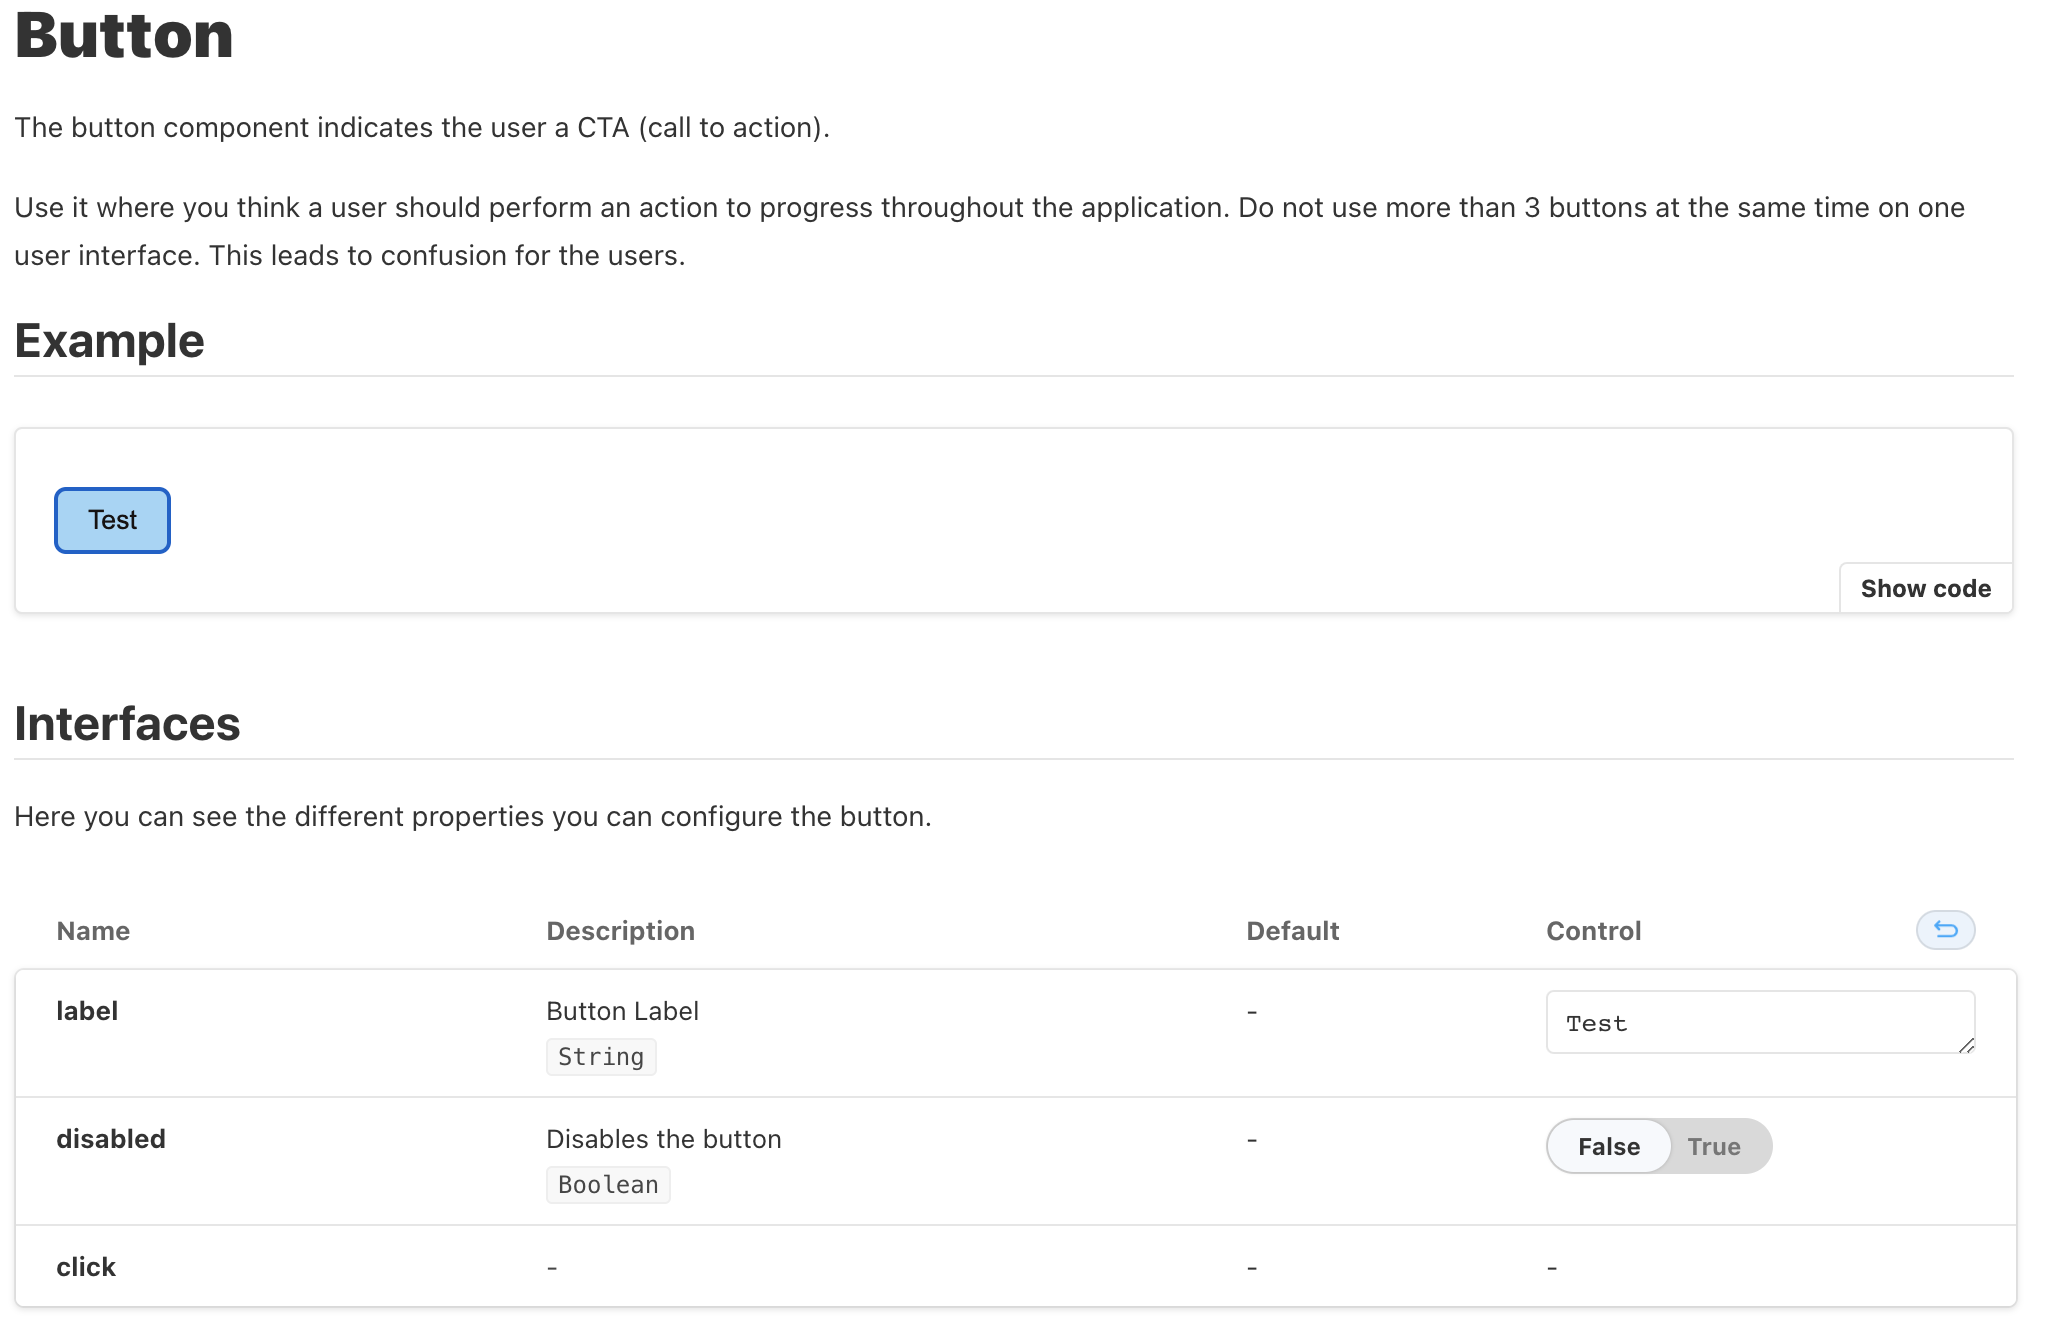
\includegraphics[width=\linewidth]{images/storybook_button.png}}
    \caption{Example documentation of the \ac{SDS} button component}
    \label{storybook_button}
\end{figure}
At the moment, the documentation consists of a short description that briefly explains to the developer how and where he can use the button in his applications. In addition, a live example of the component is presented, which is automatically linked to the properties shown below. When the properties are changed, the example above is updated. This means that the developer or designer who wants to use this component can find out which configuration is most suitable for his use cases. \\
Inspecting the DOM element of the button component, the element explorer looks like Figure \ref{button_element_explorer}. When you create a new web component, the saas-button tag is a valid DOM element. A new shadow root is opened inside the button component. This allows the web component to isolate styles and elements from the global document. The elements used to display the button component are defined in this shadow root. Also, the styles for the button are defined at the shadow DOM level, so the rest of the DOM tree never receives these styles. This helps to keep elements and styles separated and easy to understand. \\
\begin{figure}[htbp]
    \centerline{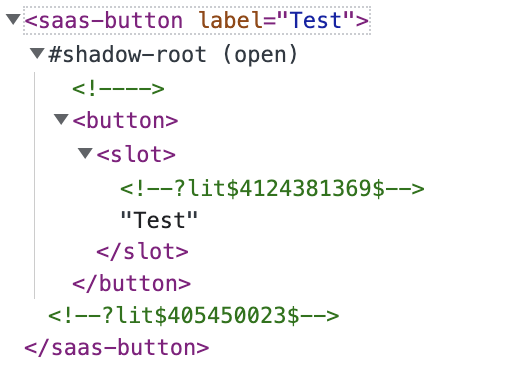
\includegraphics[height=100px]{images/button_element_explorer.png}}
    \caption{Inspection of \ac{SDS} button in elelement explorer}
    \label{button_element_explorer}
\end{figure}
It is important that \ac{CSS} variables declared in the root of the document are also available in the shadow DOM. In contrast, style declarations, e.g. for the button element in the overall document, are not applied to DOM elements in the shadow DOM. \\
The \texttt{<slot>} element in the shadow DOM is a default placeholder for anything that is inserted into the \texttt{<saas-button>} element when using the web component. The content is projected within the shadow DOM and inserted in place of the \texttt{<slot>} element. This makes it possible to create nested elements with web components which is useful in many different use cases. \\

The example of a simple button component shows how to create and use the components of \ac{SDS}. From here it is trivial to build all the different components needed to create patterns. This is because patterns, as described, are a combination of components that can be reused in applications. The missing piece to using the \ac{SDS} in an application is integration, which is explained in the next chapter.